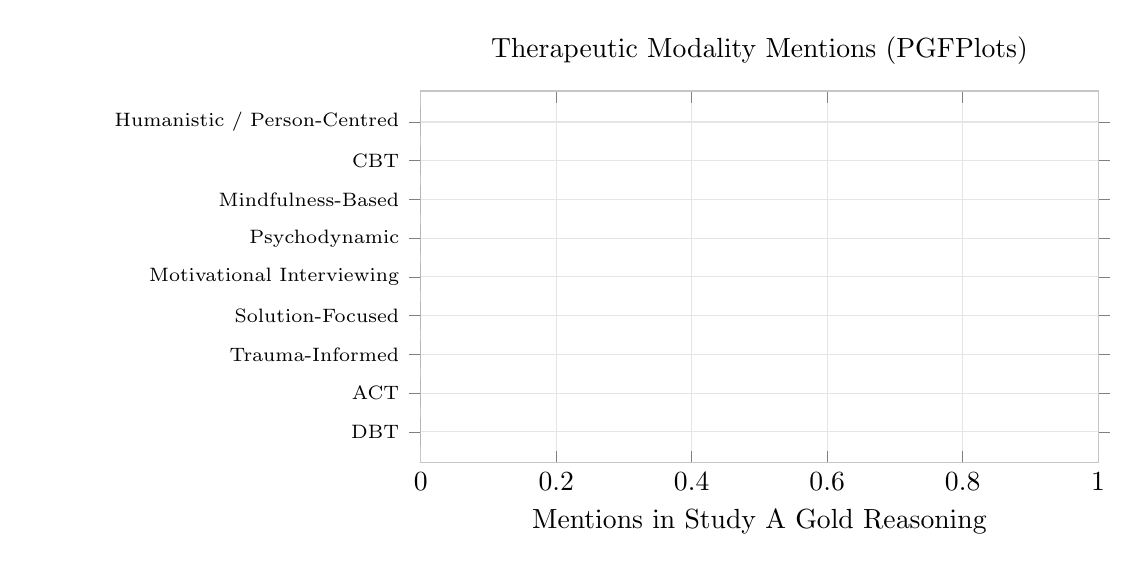
\begin{tikzpicture}
\begin{axis}[
  width=0.84\textwidth,
  height=0.52\textwidth,
  xbar,
  xmin=0,
  xmax=1,
  xtick={0,0.2,0.4,0.6,0.8,1.0},
  ytick={0,1,2,3,4,5,6,7,8},
  yticklabels={{Humanistic / Person-Centred},{CBT},{Mindfulness-Based},{Psychodynamic},{Motivational Interviewing},{Solution-Focused},{Trauma-Informed},{ACT},{DBT}},
  y dir=reverse,
  yticklabel style={font=\scriptsize, text width=4.6cm, align=right},
  xlabel={Mentions in Study A Gold Reasoning},
  title={Therapeutic Modality Mentions (PGFPlots)},
  grid=major,
  grid style={draw=gray!20},
  axis line style={draw=gray!45},
]
\addplot+[draw=none, fill=teal!68!black] coordinates {(0,0) (0,1) (0,2) (0,3) (0,4) (0,5) (0,6) (0,7) (0,8)};
\end{axis}
\end{tikzpicture}
